\documentclass[12pt,fleqn]{article}

\usepackage[english]{babel}
\usepackage{SpeedyGonzales}
\usepackage{MediocreMike}
\usepackage{Blastoise}

\usepackage[backend=biber, style=alphabetic, citestyle=alphabetic, maxcitenames=4, maxbibnames=4, mincitenames=2]{biblatex}

\title{Synthesising Abstract Deep Computer Vision Pretraining Data}

\author{Søren Winkel Holm, s183911}
\date{\today}

\pagestyle{fancy}
\fancyhf{}
\lhead{02561 Computer Graphics}
\chead{}
\rhead{Technical University of Denmark}
\lfoot{Final Project: Synthetic Computer Vision Data}
\rfoot{Page \thepage{} of \pageref{LastPage}}

\graphicspath{{imgs/}}
\linespread{1.15}
\addbibresource{references.bib}

\begin{document}

\maketitle
\thispagestyle{fancy}
\tableofcontents
\newpage

\section{Introduction}%
\label{sec:intro}
In the field of computer vision, large deep learning models have become the norm for solving semantic classification problems such image segmentation.
These performant methods have some central problems:
First of, to start training them, a larger number of images are required with corresponding manually annotated ground truth labels which are costly.
Secondly, the training proces takes takes a long time and is compute expensive as the model iteratively has to reach convergence from a starting point of randomly initialized parameters.
Finally, the error modes and interpretations of results are notoriously difficult.

A possible tool to mitigate these issues is the use of synthetic data.
If models could learn generalizable parametrizations from cheap, computer generated images, the amount of real world data and case by case training time would be reduced.
Synthetic data could also help to interpret model performance as the generated scenes can be designed to reveal flaws.

For this idea to work, the generated scenes should contain discernable objects and the learning task should require that the model converge to some representations of fundamental principles of object detection.
These principles could serve as inductive biases to help the model on real-world tasks.
One such principle is the modelling of object texture where the model should be able to map local visual patterns to class attributions.

In this project, I will explore an approach to generating such a synthetic dataset and perform tests of applying this dataset to a real-world use case.
I explore using noise functions to give the objects variations in texture connected to class assignments.

\section{Methods}%
\label{sec:method}
All code is available with reproduction instructions on \href{https://github.com/sorenmulli/imgseg-fake-balloons}{github.com/sorenmulli/imgseg-fake-balloons} and the WebGL renders can be seen on \href{https://www.student.dtu.dk/~s183911/proj/webgl-site/index.html}{student.dtu.dk/~s183911/proj/webgl-site}.
\subsection{Synthetic Scene Rendering}
\paragraph{Task 1: Noise Functions and The Simple Scene}
In the fragment shader, two noise functions were implemented, both accepting three-dimensional vector input.
\begin{enumerate}
    \item Improved Perlin noise (PN) using a permutation polynomial as \citeauthor{mcewan2012efficient} \cite{mcewan2012efficient}. 3D PN chooses pseudo-random gradients $\in \RR^3$ at regular grid points in each axis, interpolating a smooth function consistent with the gradients \cite{gustavson2005simplex}. 
    \item Sparse convolution noise (SC) as \citeauthor{frisvad2007fast} \cite{frisvad2007fast}. SC targets minimal artifacts or patterns by approximates the computationally expensive white noise filtered with a Gaussian kernel using a cubic kernel instead.
\end{enumerate}
Changing magnitude of the input vector -- the point at which the noise landscape is queried -- is equivalent to controlling the zoom level of the noise texture.
The implementations were largely based on reference implementations \cite{frisvad2016exploring}:
Only minor code changes and commenting were performed along with using the functions to texture the scene objects with a given noise scale $r$.

An initial scene was constructed by rendering a coloured sphere through 5-fold recursive subdivision of tetrahedra.
This foreground object was shaded using Phong shading from a positional light behind a perspective camera.
The object was textured using the noise functions evaluated at normals scaled with a free parameter called noise scale.
This texturing was perform by letting the noise intensity controlling the diffuse light intensity, see Listing \ref{lst:light}.

Behind the object, a 2D noise textured background in black and white was placed.

The resulting scene can bee seen at Figure \ref{fig:t1} and the noise function and other variables can be user controlled on Page \href{https://www.student.dtu.dk/~s183911/proj/webgl-site/t1.html}{t1.html}.
\lstinputlisting[language=C, firstline=134, lastline=146, caption=Fragment shader snippet related to texturing of foreground objects, label=lst:light]{../webgl-site/t1.html}

\paragraph{Task 2: Random Scenes}
The simple scene was extended to rendering multiple objects.
To generate a scene, the number of objects to generate $1 \le N \le 20 $ and the background noise scale $r_\text{background} \in [1, 20]$ were randomly, uniformly chosen.
For each of the $N$ objects, the scale, $(x, y)$-position and a number of lighting parameters were randomly chosen; see Listing \ref{lst:sphere}.

The randomly generated scenes can be seen and object variables controlled on Page \href{https://www.student.dtu.dk/~s183911/proj/webgl-site/t2.html}{t2.html}.
\lstinputlisting[language=javascript, firstline=36, lastline=44, caption=Javascript code snippet with random variable generation run for each object, label=lst:sphere]{../webgl-site/randomness.js}
\paragraph{Task 3: Object Classes}
Three parameters controlling characteristics of each object were not set by the random scene and were instead set based on object class
\begin{itemize}
    \item Colour Hue $h \in [0, 360]$. The emitted radiance of each object was chosen in HSL-format to be $(h, 1, 0.5)$ and converted to RGB. Thus, all objects had fixed lightness and fully saturated colours (before texturing with noise and shading by light) motivated to get a single value expressing most of the dynamics in colour.
    \item Object elongation $\rho \in [0, 1]$. When $\rho\ne \half$, the object is subject to axis parallel scaling, converting spheres to ellipsoids. 
        Higher $\rho$ means a wider ($x$-elongated) object and the implementation can be seen in Listing \ref{lst:elongation}.
    \item The noise scale $r > 1$ used to texture the object.
\end{itemize}
Three classes of objects where implemented and to each class was attributed an average values for each of the above characteristics, making class $i$ be described by $(h_k, \rho_k, r_k)$.
The chosen values can be seen in Table \ref{tab:class-avg} and the objects rendered with the average characteristics can be seen in Figure \ref{fig:t3}.
\begin{table}[H]
    \centering
        \begin{tabular}{l|lll}
            Class $k$ & $h_k$ & $\rho_k$ & $r_k$ \\
            \hline
            1 & 150 & $0.55$ & $5$ \\
            2 & 250 & $0.45$ & $17.5$ \\
            3 & 350 & $0.5$ & $30$
        \end{tabular}
    \caption{
        The average value in each class prior for hue, elongation and noise scale.
    }
    \label{tab:class-avg}
\end{table}\noindent
Each object was randomly assigned one of the three classes with equal probability.
When rendering an object, random values of $h, \rho, r$ were chosen based on the object class according to the Gaussians
\begin{equation}
    h \sim \mathcal N\left( h_k, 50^2 \right),
    \rho \sim \mathcal N\left( \rho_k, 0.05^2 \right),
    r \sim \mathcal N\left( r_k, 5^2 \right).
\end{equation}
After drawing these values, the sphere characteristics were set after enforcing the variable ranges; for $\rho, r$ by clamping to borders and for $h$, by taking modulo 360.

These random object realisations influenced by by class prior of assigned classes can be sampled on Page \href{https://www.student.dtu.dk/~s183911/proj/webgl-site/t3.html}{t3.html} with some examples shown in Appendix \ref{sec:cls}.

\lstinputlisting[language=javascript, firstline=65, lastline=70, caption=Javascript code snippet which produces the tranformation matrix to elongate the objects according to $\rho$. This matrix is incorporated into the model matrix for this specific object., label=lst:elongation]{../webgl-site/sphere.js}
\paragraph{Task 4: The Full Scene With Label Maps}
To generate training data, each image must have a corresponds target representing the ground truth of the task.
For image segmentation, this ground truth should be a pixel map representing the class label of the object visible in the image at that pixel.

This was done in WebGL by adding a separate rending mode where the fragment colour had hue $h_k$ when drawing an object with class $k$, bypassinng all texturing and lighting calculations.
The background is rendered black, giving four unique pixel values representing four labels\footnote{Pixels at the borders of objects were blended by the fragment shader giving some extra values. These were ignored when loading the dataset into Python, only accepting the object interior as corresponding to class $k$}.

This feature was combined with the class assignments in Task 3 and the random scenes from Task 2 to producgtGe synthetic scenes with class assigned objects and corresponding label maps.
One example of such as pair shown in \ref{fig:t4} and another in Appendix \ref{sec:appt4}.

The ability to download the rendered scene was added, and each rendering was given a random string as output name to be able to match images and label maps.
This final interface is available on Page \href{https://www.student.dtu.dk/~s183911/proj/webgl-site/t4.html}{t4.html}.

\paragraph{Generated Datasets}
To extract a dataset from the WebGL application, dynamic website scraping was implemented in \code{Python} using a Selenium headless Firefox web browser \cite{selenium2022docs}.
$10,000$ pairs of $512\times 512$ images and corresponding label maps were extracted textured with PN and another $10,000$ with SC, requiring the rendering of $40,000$ images, which took around five hours on a consumer CPU.
The two datasets were called \texttt{perlin} and \texttt{sc} and can be downloaded through links on the GitHub repository.

\subsection{Deep Image Segmentation}
\paragraph{Baseline Learning Task}
The chosen benchmark task was image segmentation, also called semantic segmentation or pixel wise object detection, where the algorithm should classify each pixel according to visible object class, segmenting the image into bounded, semantic regions \cite{stockman2001cv}. 
As benchmark dataset, the Common Objects in Context (COCO) 2017 Object Detection Dataset was chosen which is a collection of every day photographs with object annotations in over 80 categories \cite{lin2014coco}.
A subset of 20 foreground classes including \emph{person}, \emph{car} and \emph{dog} as was chosen for the learning benchmark in accordance with the PyTorch Torchvision image segmentation reference \cite{falbel2022torch}.

Images without objects in these classes were discarded.
To keep computational scope down and simulate the data limited learning case, the large dataset was subsampled to $1,000$ training images and $1,000$ validation images.

The machine learning model to map from images to segmentation label maps had the architecture of a Fully-Convolutional Deep Neural Network with a ResNet-50 backbone as described by \citeauthor{shelhamer2017fully} \cite{shelhamer2017fully}.

The COCO training set was used for optimization using stochastic gradient descent for 10 epochs, evaluating generalization performance to the validation set each epoch, using direct accuracy, Intersection-over-union (IoU, also called Jaccard Index) and F1-score \cite{moral2019new}.
Note that, in this multiclass setting, all these scores have two different approaches to computation: Macro which produces the final score by a simple average of scores for each class, and micro averaging which averages class performance by class frequency.
In a class imbalanced problem dominated by a single class such as image segmentation with a background class, macro average scores can be expected to be lower.

The training was performed on a Nvidia A100 GPU and took about half an hour.

\paragraph{Training on Synthetic Data}
For each of the two synthetic datasets, \texttt{perlin} and \texttt{sc}, a tenth of the data was set aside for validating performance and training of a model was performed on the 9000 images exactly as above for 30 epochs, taking $3.5$ hours.


\paragraph{Transfer learning of Pretrained Model}
To test the usefulness of the synthetic data for practical image segmentation, the model was after training on synthetic data adapted to the COCO task using the paradigm of transformer learning.
In this context, the synthetic data training is the pretraining step and the COCO benchmark is the downstream or finetuning task.

This was done by augmenting the training on COCO by initializing the model weights from the network converged on the synthetic dataset instead of random initialization.
The final layers, the classification head, which are dependant on the number of classes and thus cannot be shared between $4$-class and $21$-class segmentation tasks cannot be transferred.

\section{Results}%
\label{sec:results}
\begin{figure}[H]
    \centering
        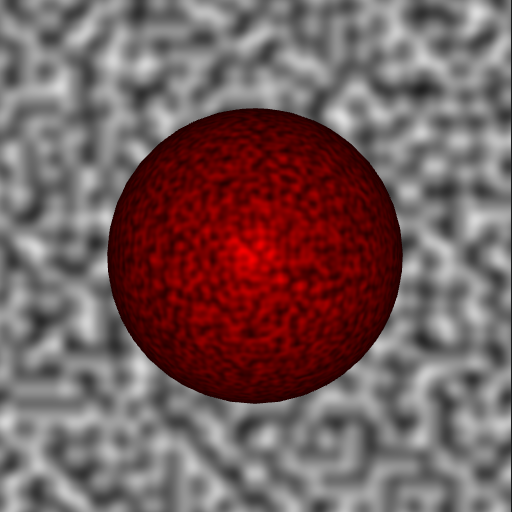
\includegraphics[width=.48\linewidth]{t1-perlin}
        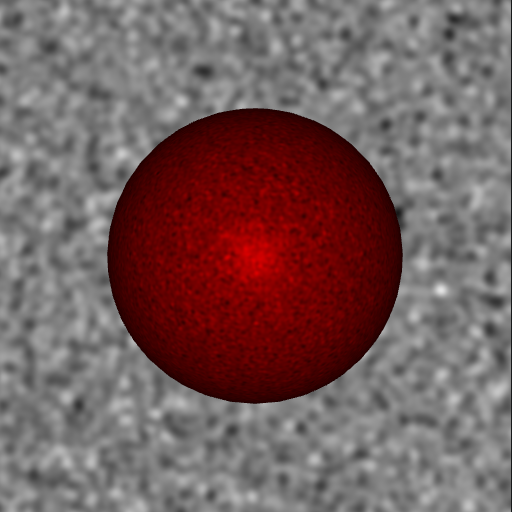
\includegraphics[width=.48\linewidth]{t1-sc}
    \caption{
        The Task 1 image where the scene is textured using PN (left) and SC (right); both with a noise scale of 25.
    }
    \label{fig:t1}
\end{figure}\noindent

\begin{figure}[H]
    \centering
        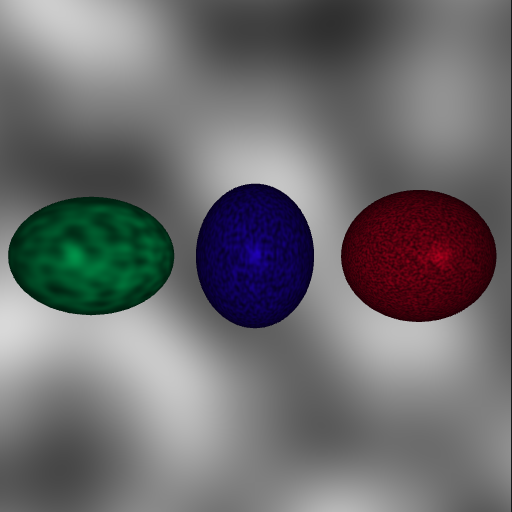
\includegraphics[width=.48\linewidth]{t3-avg-perlin}
        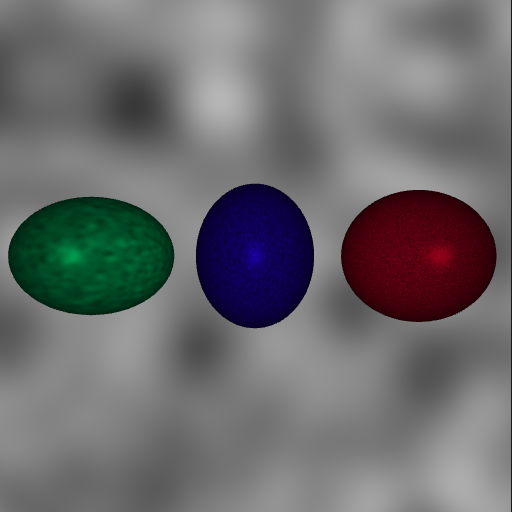
\includegraphics[width=.48\linewidth]{t3-avg-sc}
    \caption{
       Task 3 images showing the class prototype for each class from left to right in both PN (left) and SC (right).
       These spheres thus have their elongation $\rho$, noise scale $r$ and hue $h$ set to the class averages.
       To see examples of variation within classes, see Appendix \ref{sec:cls}.
    }
    \label{fig:t3}
\end{figure}\noindent

\begin{figure}[H]
    \centering
        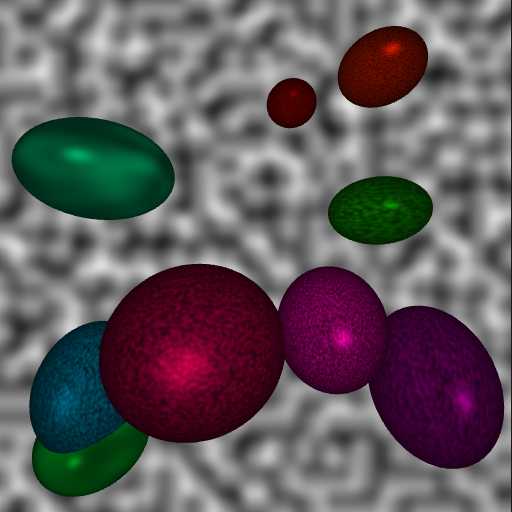
\includegraphics[width=0.49\linewidth]{t4-img}
        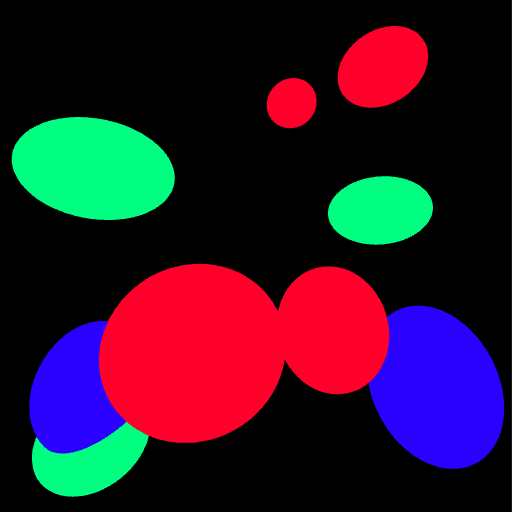
\includegraphics[width=0.49\linewidth]{t4-labelmap}
    \caption{
        The final Task 4 result.
        Left: A random scene with class assigned objects textured with PN. Right: The corresponding ground truth class labels where green is class 1, blue class 2 and red class 3.
    }
    \label{fig:t4}
\end{figure}\noindent

\begin{figure}[H]
    \centering
        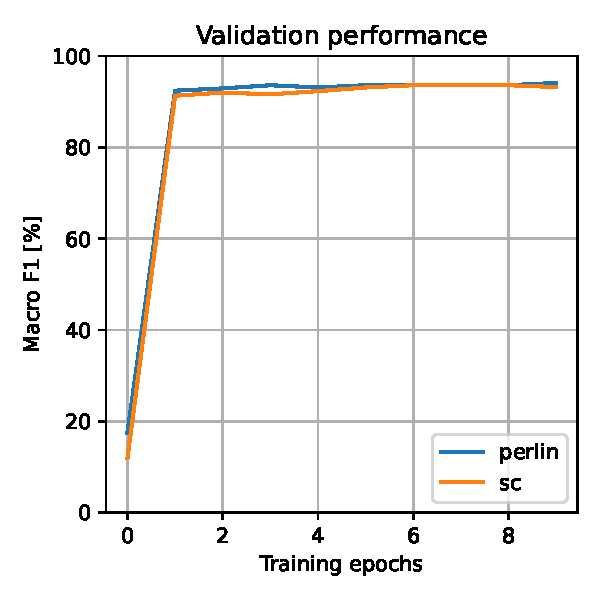
\includegraphics[width=.49\linewidth]{fb/Macro F1}
        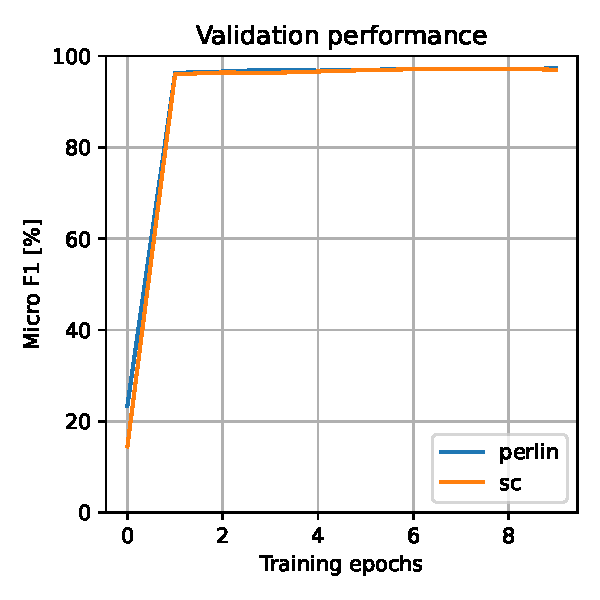
\includegraphics[width=.49\linewidth]{fb/Micro F1}
    \caption{
        F1 scores on validation datasets, with macro (left) and micro (right) averaging, during training of the two synthetic datasets. See Appendix \ref{sec:apptrain} for these curves with other measures.
    }
    \label{fig:fbcurves}
\end{figure}\noindent


\begin{table}[H]
    \small
    \centering
    \begin{tabular}{l|llllll}
            Method & Micro Accuracy & Macro Accuracy & Micro IoU & Macro IoU & Micro F1 & Macro F1 \\
            \hline
            perlin & $97 \pm 1$ & $93 \pm 2$ & $94 \pm 2$ & $88 \pm 2$ & $97 \pm 1$ & $93 \pm 2$ \\
            sc & $97 \pm 1$ & $94 \pm 2$ & $94 \pm 1$ & $88 \pm 2$ & $97 \pm 1$ & $93 \pm 2$ \\
    \end{tabular}
    \caption{
        Validation results after the final epoch of training on the synthetic datasets with $\alpha=5\pro$ confidence intervals according to large sample normality assumption for proportions \cite[Method 7.3]{brock2015intro}.
    }
    \label{tab:fbfinal}
\end{table}\noindent

\begin{figure}[H]
    \centering
        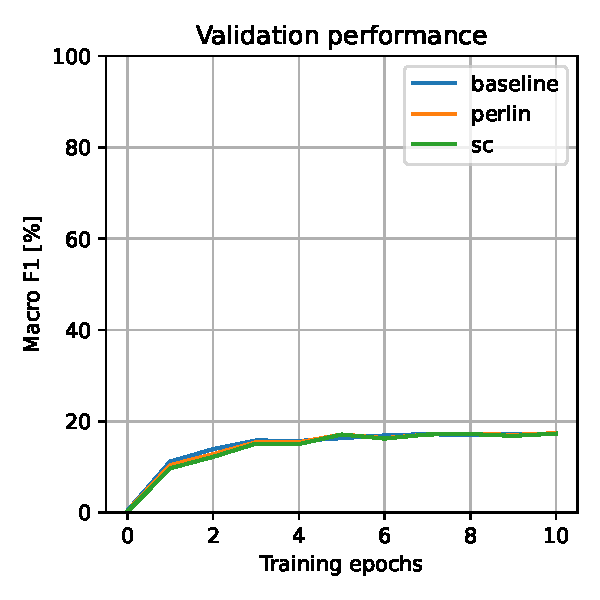
\includegraphics[width=.49\linewidth]{coco/Macro F1}
        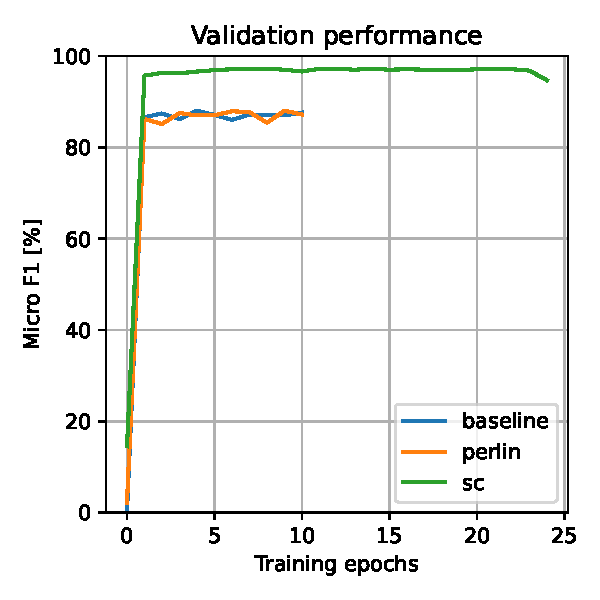
\includegraphics[width=.49\linewidth]{coco/Micro F1}
    \caption{
        Macro, micro F1 scores on the COCO validation set during training of the COCO benchmark with different model initializations. Baseline corresponds to training from newly initialized models and the other two to transfer learning from models pretrained from each dataset. See Appendix \ref{sec:apptrain} for these curves with other measures.
    }
    \label{fig:cococurves}
\end{figure}\noindent


\begin{table}[H]
    \small
    \centering
    \begin{tabular}{l|llllll}
            Method & Micro Accuracy & Macro Accuracy & Micro IoU & Macro IoU & Micro F1 & Macro F1 \\
            \hline
            baseline & $88 \pm 2$ & $17 \pm 2$ & $78 \pm 3$ & $14 \pm 2$ & $88 \pm 2$ & $17 \pm 2$ \\
            perlin & $87 \pm 2$ & $17 \pm 2$ & $78 \pm 3$ & $14 \pm 2$ & $87 \pm 2$ & $17 \pm 2$ \\
            sc & $95 \pm 1$ & $88 \pm 2$ & $90 \pm 2$ & $79 \pm 3$ & $95 \pm 1$ & $87 \pm 2$ \\
    \end{tabular}
    \caption{
        COCO final validation results for three initialization approaches.
    }
    \label{tab:fbfinal}
\end{table}\noindent

%TODO: Comment directly on model differences.
\section{Discussion}%
\label{sec:disc}
Initially, based on the COCO results, I must concede that I could not show what I hoped for:
That the pretraining on the synthetic dataset on different balloon-looking objects improved convergence speed or final performance.
The synthetic learning task was, however, succesful:
For both noise functions, the model converged to high performance.
Should this be taken as a sign that different computer vision tasks follow so diverging data distributions that current models cannot extract generalizable patterns across tasks?
This question deserves serious work, but I would imagine that a similar setup as this one can succeed.

Looking back, the choice of the COCO task, which appears widely used for benchmarking state of the art models, might be problematic for this project as COCO is a complex image segmentation benchmark with an incredibly variant dataset.
Improved convergence through synthetic pretraining might appear if more care is taken to the machine learning part of the project but I would first try with simpler benchmarks such as medical imaging.
Another way to improve the impact of pretraining is to improve the realism of the scenes.
Adding shadows, adding a physical world with meaningful geometry instead of floating foreground objects and adding different objects than spheres are all within reason with the methods from the course.

Regardless on the relevance for the downstream COCO task, I still find value in the dataset because it allows for the model to converge to reliable class predictions on the synthetic dataset itself.
This fact can be used to gain insights into model behaviour which would be my next step if the deadline was a week later:
How would the model F1 score change if the objects are not textured using noise functions at all?
What if they all have the same colour or same elongation?
This approach of model interpretability using synthetic data might hold much promise for deep learning.

\clearpage

\printbibliography[heading=bibintoc]

\clearpage

\appendix
\section{Additional Example Images}
\subsection{Class examples}\label{sec:cls}
See Figure \ref{fig:t3-rand-perlin} for four random instances of object classes using PN and Figure \ref{fig:t3-rand-sc} for the same using SC.
\begin{figure}[H]
    \centering
        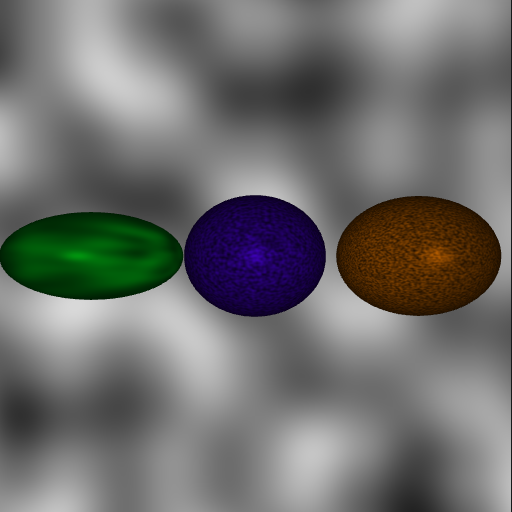
\includegraphics[width=.49\linewidth]{t3-rand1-perlin}
        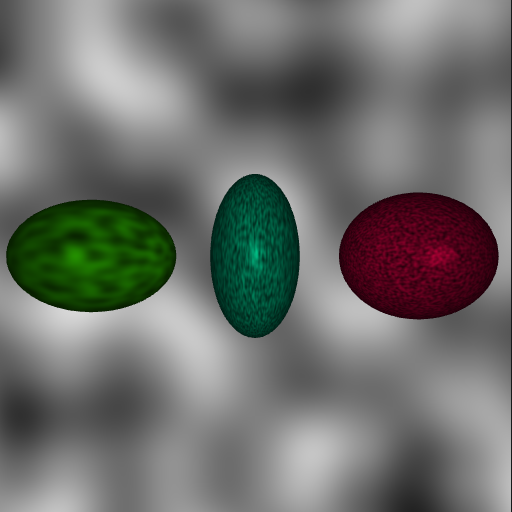
\includegraphics[width=.49\linewidth]{t3-rand2-perlin}
        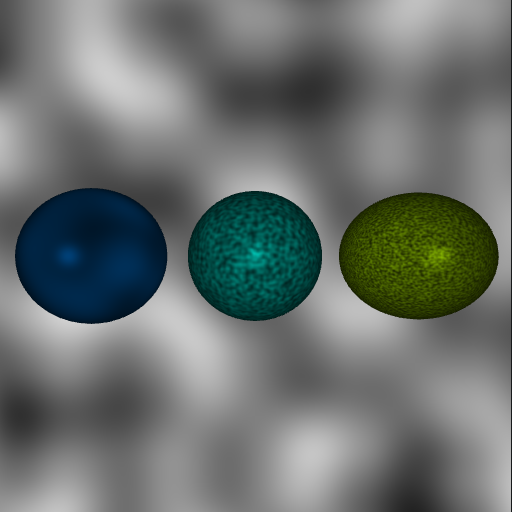
\includegraphics[width=.49\linewidth]{t3-rand3-perlin}
        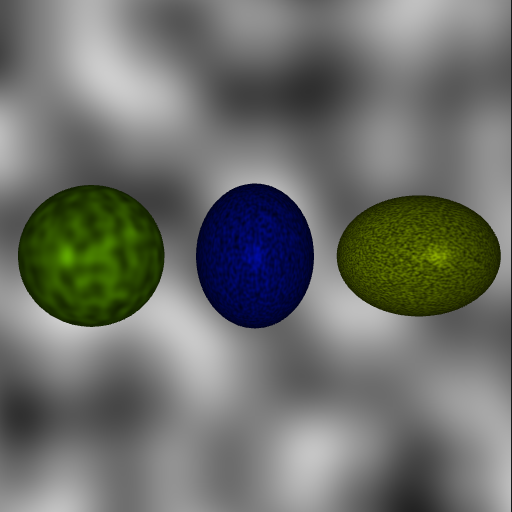
\includegraphics[width=.49\linewidth]{t3-rand4-perlin}
    \caption{
        Random instances of classes 1, 2, 3 textured using PN.
    }
    \label{fig:t3-rand-perlin}
\end{figure}\noindent

\begin{figure}[H]
    \centering
        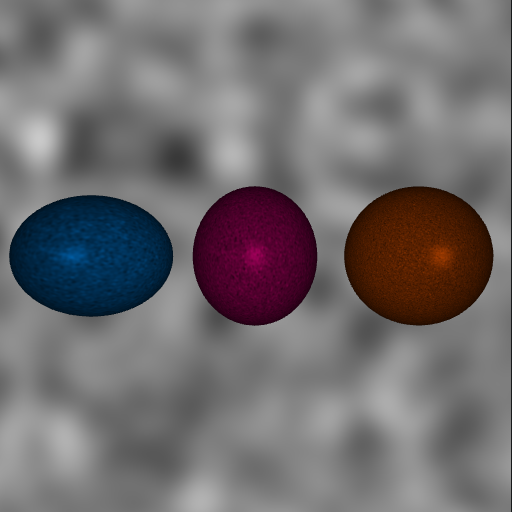
\includegraphics[width=.49\linewidth]{t3-rand1-sc}
        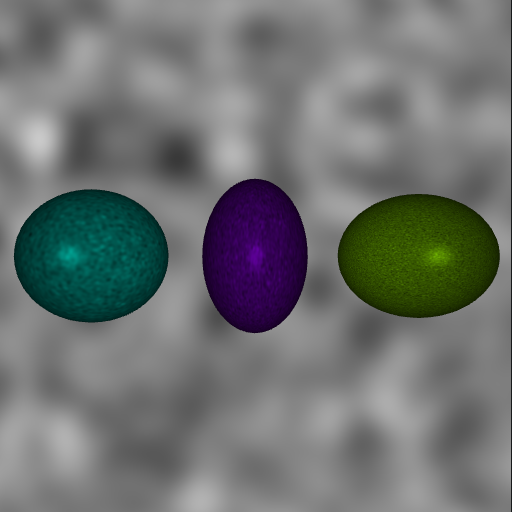
\includegraphics[width=.49\linewidth]{t3-rand2-sc}
        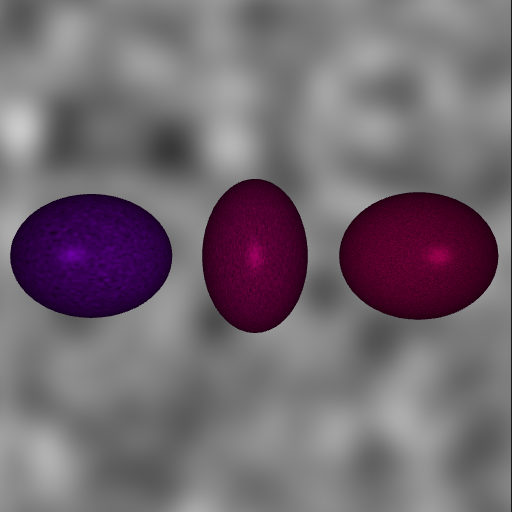
\includegraphics[width=.49\linewidth]{t3-rand3-sc}
        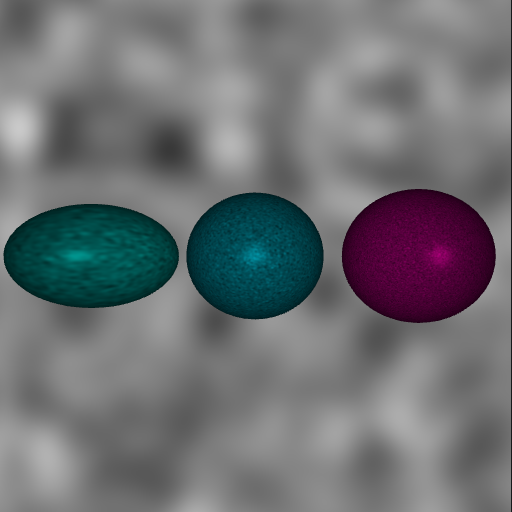
\includegraphics[width=.49\linewidth]{t3-rand4-sc}
    \caption{
        Random instances of classes 1, 2, 3 textured using SC.
    }
    \label{fig:t3-rand-sc}
\end{figure}\noindent


\subsection{Full Scenes in Different Noise Functions}\label{sec:appt4}
\begin{figure}[H]
    \centering
        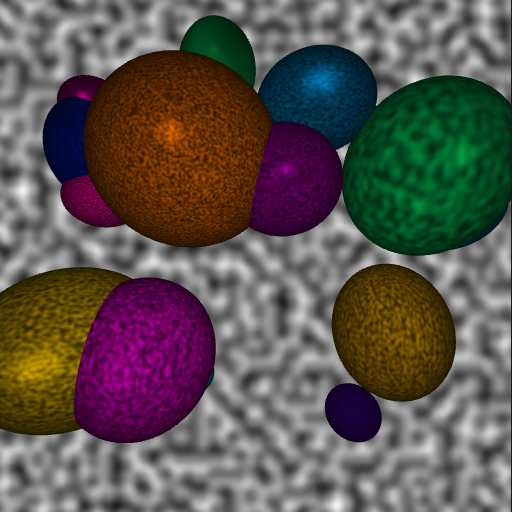
\includegraphics[width=.49\linewidth]{scene-example-perlin}
        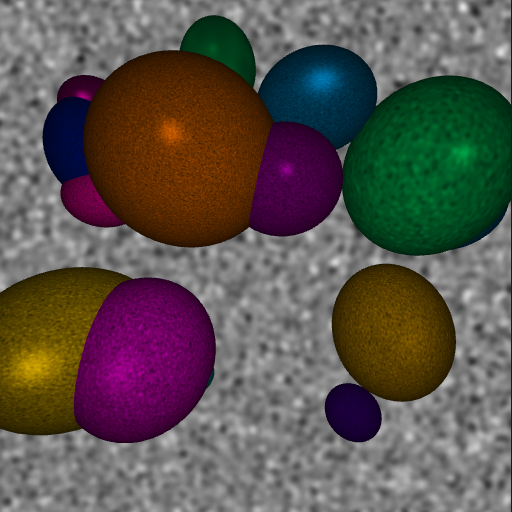
\includegraphics[width=.49\linewidth]{scene-example-sc}
        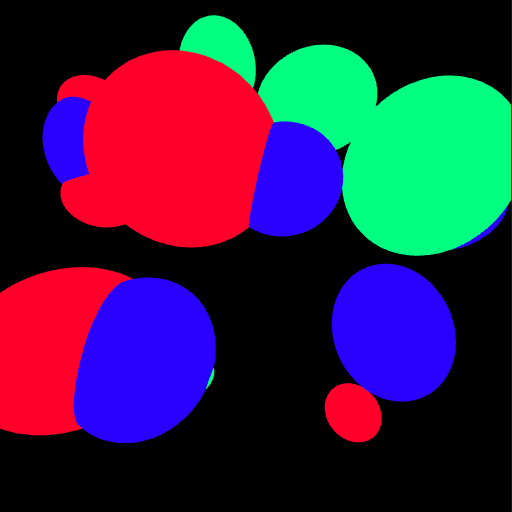
\includegraphics[width=.49\linewidth]{scene-example-labelmap}
        \caption{A random scene generated as in Task 4 with both PN (upper left) and SC (upper right).}
    \label{fig:appt4}
\end{figure}\noindent



\section{More Training Curves}\label{sec:apptrain}

\begin{figure}[H]
    \centering
        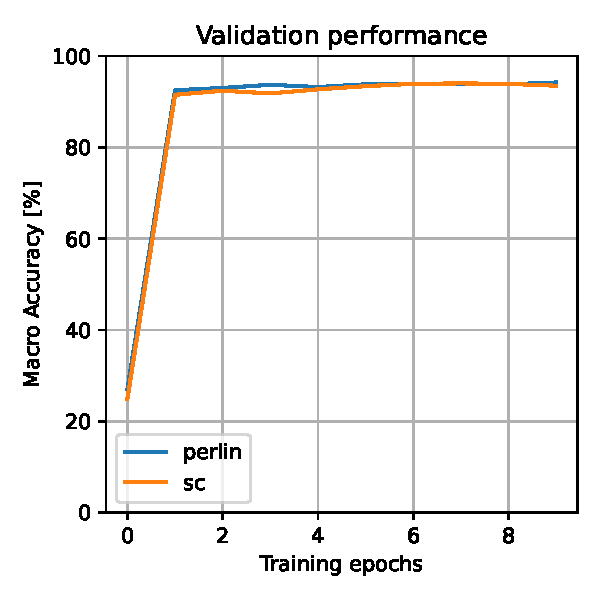
\includegraphics[width=.49\linewidth]{fb/Macro Accuracy}
        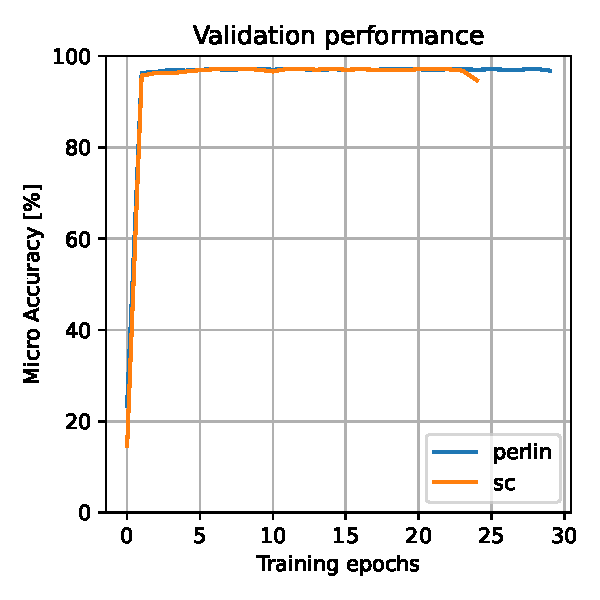
\includegraphics[width=.49\linewidth]{fb/Micro Accuracy}
        \includegraphics[width=.49\linewidth]{fb/Macro Iou}
        \includegraphics[width=.49\linewidth]{fb/Micro Iou}
    \caption{
        COCO validation scores as on figure \ref{fig:cococurves} just with the other metrics which can be seen on the $y$-axis.
    }
\end{figure}\noindent

\begin{figure}[H]
    \centering
        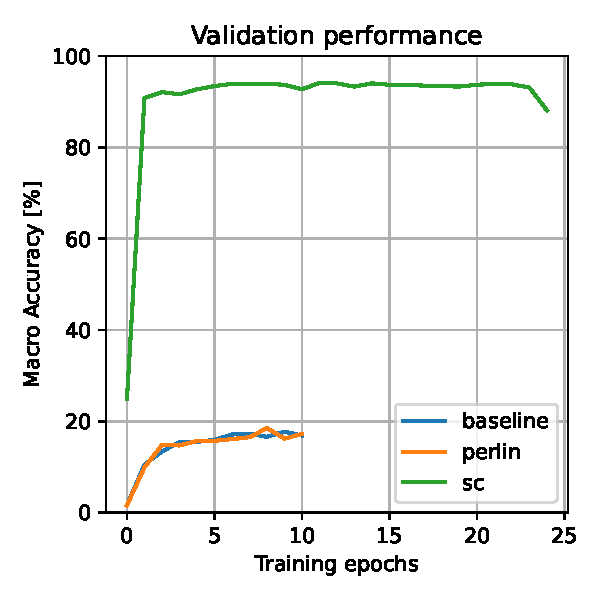
\includegraphics[width=.49\linewidth]{coco/Macro Accuracy}
        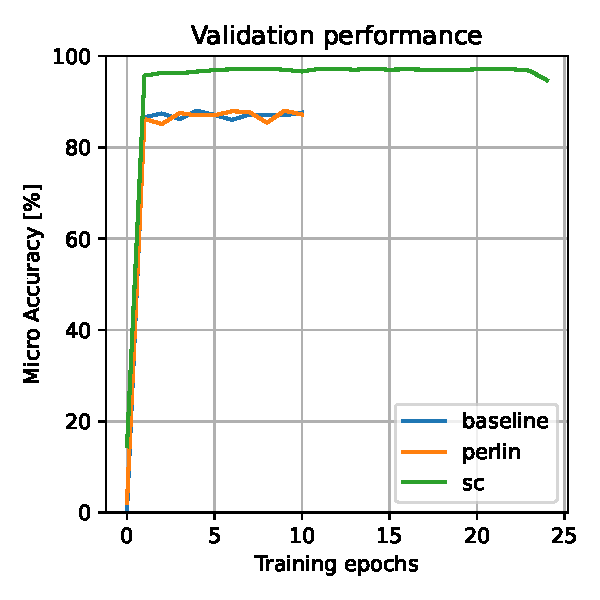
\includegraphics[width=.49\linewidth]{coco/Micro Accuracy}
        \includegraphics[width=.49\linewidth]{coco/Macro Iou}
        \includegraphics[width=.49\linewidth]{coco/Micro Iou}
    \caption{
        COCO validation scores as on figure \ref{fig:cococurves} just with the other metrics which can be seen on the $y$-axis.
    }
\end{figure}\noindent

\end{document}

